% Created by tikzDevice version 0.6.2-92-0ad2792 on 2013-11-12 07:32:35
% !TEX encoding = UTF-8 Unicode
\documentclass[12pt, mainfont = Minion,     mainscale = 1.0, sansfont = Myriad,     sansscale = MatchLowercase, monofont = Consolas,   monoscale = MatchLowercase, mathfont = MinionMath, mathscale = 1.0]{mtikzfig}
\begin{document}

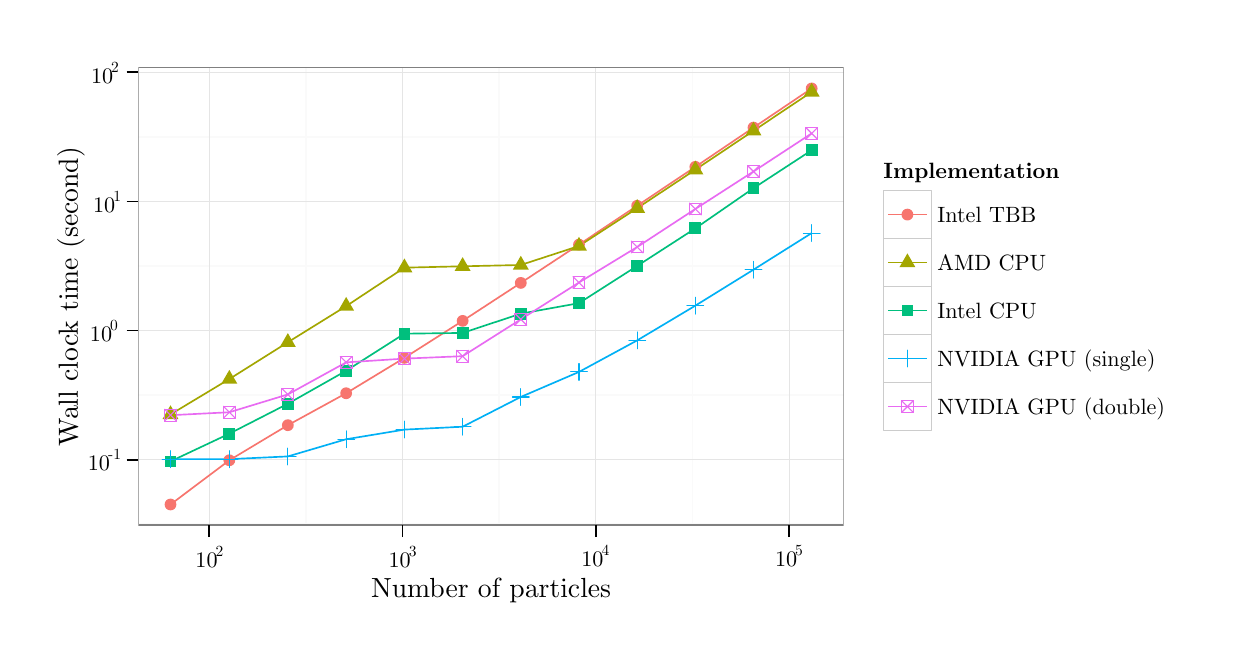
\begin{tikzpicture}[x=1pt,y=1pt]
\definecolor[named]{fillColor}{rgb}{1.00,1.00,1.00}
\path[use as bounding box,fill=fillColor,fill opacity=0.00] (0,0) rectangle (433.62,216.81);
\begin{scope}
\path[clip] (  0.00,  0.00) rectangle (433.62,216.81);
\definecolor[named]{drawColor}{rgb}{1.00,1.00,1.00}
\definecolor[named]{fillColor}{rgb}{1.00,1.00,1.00}

\path[draw=drawColor,line width= 0.6pt,line join=round,line cap=round,fill=fillColor] ( -0.00,  0.00) rectangle (433.62,216.81);
\end{scope}
\begin{scope}
\path[clip] ( 40.02, 37.00) rectangle (294.88,202.36);
\definecolor[named]{fillColor}{rgb}{1.00,1.00,1.00}

\path[fill=fillColor] ( 40.02, 37.00) rectangle (294.88,202.36);
\definecolor[named]{drawColor}{rgb}{0.98,0.98,0.98}

\path[draw=drawColor,line width= 0.6pt,line join=round] ( 40.02, 37.36) --
	(294.88, 37.36);

\path[draw=drawColor,line width= 0.6pt,line join=round] ( 40.02, 84.03) --
	(294.88, 84.03);

\path[draw=drawColor,line width= 0.6pt,line join=round] ( 40.02,130.71) --
	(294.88,130.71);

\path[draw=drawColor,line width= 0.6pt,line join=round] ( 40.02,177.38) --
	(294.88,177.38);

\path[draw=drawColor,line width= 0.6pt,line join=round] (100.53, 37.00) --
	(100.53,202.36);

\path[draw=drawColor,line width= 0.6pt,line join=round] (170.35, 37.00) --
	(170.35,202.36);

\path[draw=drawColor,line width= 0.6pt,line join=round] (240.18, 37.00) --
	(240.18,202.36);
\definecolor[named]{drawColor}{rgb}{0.90,0.90,0.90}

\path[draw=drawColor,line width= 0.2pt,line join=round] ( 40.02, 60.70) --
	(294.88, 60.70);

\path[draw=drawColor,line width= 0.2pt,line join=round] ( 40.02,107.37) --
	(294.88,107.37);

\path[draw=drawColor,line width= 0.2pt,line join=round] ( 40.02,154.04) --
	(294.88,154.04);

\path[draw=drawColor,line width= 0.2pt,line join=round] ( 40.02,200.72) --
	(294.88,200.72);

\path[draw=drawColor,line width= 0.2pt,line join=round] ( 65.62, 37.00) --
	( 65.62,202.36);

\path[draw=drawColor,line width= 0.2pt,line join=round] (135.44, 37.00) --
	(135.44,202.36);

\path[draw=drawColor,line width= 0.2pt,line join=round] (205.27, 37.00) --
	(205.27,202.36);

\path[draw=drawColor,line width= 0.2pt,line join=round] (275.09, 37.00) --
	(275.09,202.36);
\definecolor[named]{drawColor}{rgb}{0.97,0.46,0.43}

\path[draw=drawColor,line width= 0.6pt,line join=round] ( 51.61, 44.51) --
	( 72.87, 60.49) --
	( 94.01, 73.17) --
	(115.08, 84.71) --
	(136.13, 97.49) --
	(157.17,110.86) --
	(178.19,124.58) --
	(199.21,138.42) --
	(220.24,152.45) --
	(241.26,166.52) --
	(262.27,180.70) --
	(283.29,194.84);
\definecolor[named]{drawColor}{rgb}{0.64,0.65,0.00}

\path[draw=drawColor,line width= 0.6pt,line join=round] ( 51.61, 77.05) --
	( 72.87, 89.84) --
	( 94.01,103.13) --
	(115.08,116.19) --
	(136.13,130.09) --
	(157.17,130.58) --
	(178.19,131.06) --
	(199.21,137.91) --
	(220.24,151.58) --
	(241.26,165.49) --
	(262.27,179.55) --
	(283.29,193.59);
\definecolor[named]{drawColor}{rgb}{0.00,0.75,0.49}

\path[draw=drawColor,line width= 0.6pt,line join=round] ( 51.61, 60.08) --
	( 72.87, 70.10) --
	( 94.01, 80.91) --
	(115.08, 92.83) --
	(136.13,106.23) --
	(157.17,106.50) --
	(178.19,113.47) --
	(199.21,117.26) --
	(220.24,130.71) --
	(241.26,144.28) --
	(262.27,158.80) --
	(283.29,172.52);
\definecolor[named]{drawColor}{rgb}{0.00,0.69,0.96}

\path[draw=drawColor,line width= 0.6pt,line join=round] ( 51.61, 60.90) --
	( 72.87, 60.90) --
	( 94.01, 61.88) --
	(115.08, 68.09) --
	(136.13, 71.57) --
	(157.17, 72.61) --
	(178.19, 83.37) --
	(199.21, 92.41) --
	(220.24,103.81) --
	(241.26,116.36) --
	(262.27,129.36) --
	(283.29,142.58);
\definecolor[named]{drawColor}{rgb}{0.91,0.42,0.95}

\path[draw=drawColor,line width= 0.6pt,line join=round] ( 51.61, 76.77) --
	( 72.87, 77.84) --
	( 94.01, 84.28) --
	(115.08, 95.87) --
	(136.13, 97.22) --
	(157.17, 98.10) --
	(178.19,111.42) --
	(199.21,124.72) --
	(220.24,137.55) --
	(241.26,151.29) --
	(262.27,164.84) --
	(283.29,178.60);
\definecolor[named]{fillColor}{rgb}{0.97,0.46,0.43}

\path[fill=fillColor] ( 51.61, 44.51) circle (  2.13);
\definecolor[named]{fillColor}{rgb}{0.64,0.65,0.00}

\path[fill=fillColor] ( 51.61, 80.36) --
	( 54.48, 75.39) --
	( 48.73, 75.39) --
	cycle;
\definecolor[named]{fillColor}{rgb}{0.00,0.75,0.49}

\path[fill=fillColor] ( 49.47, 57.95) --
	( 53.74, 57.95) --
	( 53.74, 62.21) --
	( 49.47, 62.21) --
	cycle;
\definecolor[named]{drawColor}{rgb}{0.00,0.69,0.96}

\path[draw=drawColor,line width= 0.4pt,line join=round,line cap=round] ( 48.59, 60.90) -- ( 54.63, 60.90);

\path[draw=drawColor,line width= 0.4pt,line join=round,line cap=round] ( 51.61, 57.88) -- ( 51.61, 63.92);
\definecolor[named]{drawColor}{rgb}{0.91,0.42,0.95}

\path[draw=drawColor,line width= 0.4pt,line join=round,line cap=round] ( 49.47, 74.64) rectangle ( 53.74, 78.91);

\path[draw=drawColor,line width= 0.4pt,line join=round,line cap=round] ( 49.47, 74.64) -- ( 53.74, 78.91);

\path[draw=drawColor,line width= 0.4pt,line join=round,line cap=round] ( 49.47, 78.91) -- ( 53.74, 74.64);
\definecolor[named]{fillColor}{rgb}{0.97,0.46,0.43}

\path[fill=fillColor] ( 72.87, 60.49) circle (  2.13);
\definecolor[named]{fillColor}{rgb}{0.64,0.65,0.00}

\path[fill=fillColor] ( 72.87, 93.15) --
	( 75.74, 88.18) --
	( 69.99, 88.18) --
	cycle;
\definecolor[named]{fillColor}{rgb}{0.00,0.75,0.49}

\path[fill=fillColor] ( 70.73, 67.96) --
	( 75.00, 67.96) --
	( 75.00, 72.23) --
	( 70.73, 72.23) --
	cycle;
\definecolor[named]{drawColor}{rgb}{0.00,0.69,0.96}

\path[draw=drawColor,line width= 0.4pt,line join=round,line cap=round] ( 69.85, 60.90) -- ( 75.89, 60.90);

\path[draw=drawColor,line width= 0.4pt,line join=round,line cap=round] ( 72.87, 57.88) -- ( 72.87, 63.92);
\definecolor[named]{drawColor}{rgb}{0.91,0.42,0.95}

\path[draw=drawColor,line width= 0.4pt,line join=round,line cap=round] ( 70.73, 75.71) rectangle ( 75.00, 79.98);

\path[draw=drawColor,line width= 0.4pt,line join=round,line cap=round] ( 70.73, 75.71) -- ( 75.00, 79.98);

\path[draw=drawColor,line width= 0.4pt,line join=round,line cap=round] ( 70.73, 79.98) -- ( 75.00, 75.71);
\definecolor[named]{fillColor}{rgb}{0.97,0.46,0.43}

\path[fill=fillColor] ( 94.01, 73.17) circle (  2.13);
\definecolor[named]{fillColor}{rgb}{0.64,0.65,0.00}

\path[fill=fillColor] ( 94.01,106.44) --
	( 96.88,101.47) --
	( 91.13,101.47) --
	cycle;
\definecolor[named]{fillColor}{rgb}{0.00,0.75,0.49}

\path[fill=fillColor] ( 91.87, 78.77) --
	( 96.14, 78.77) --
	( 96.14, 83.04) --
	( 91.87, 83.04) --
	cycle;
\definecolor[named]{drawColor}{rgb}{0.00,0.69,0.96}

\path[draw=drawColor,line width= 0.4pt,line join=round,line cap=round] ( 90.99, 61.88) -- ( 97.02, 61.88);

\path[draw=drawColor,line width= 0.4pt,line join=round,line cap=round] ( 94.01, 58.86) -- ( 94.01, 64.90);
\definecolor[named]{drawColor}{rgb}{0.91,0.42,0.95}

\path[draw=drawColor,line width= 0.4pt,line join=round,line cap=round] ( 91.87, 82.14) rectangle ( 96.14, 86.41);

\path[draw=drawColor,line width= 0.4pt,line join=round,line cap=round] ( 91.87, 82.14) -- ( 96.14, 86.41);

\path[draw=drawColor,line width= 0.4pt,line join=round,line cap=round] ( 91.87, 86.41) -- ( 96.14, 82.14);
\definecolor[named]{fillColor}{rgb}{0.97,0.46,0.43}

\path[fill=fillColor] (115.08, 84.71) circle (  2.13);
\definecolor[named]{fillColor}{rgb}{0.64,0.65,0.00}

\path[fill=fillColor] (115.08,119.51) --
	(117.96,114.53) --
	(112.21,114.53) --
	cycle;
\definecolor[named]{fillColor}{rgb}{0.00,0.75,0.49}

\path[fill=fillColor] (112.95, 90.70) --
	(117.22, 90.70) --
	(117.22, 94.96) --
	(112.95, 94.96) --
	cycle;
\definecolor[named]{drawColor}{rgb}{0.00,0.69,0.96}

\path[draw=drawColor,line width= 0.4pt,line join=round,line cap=round] (112.07, 68.09) -- (118.10, 68.09);

\path[draw=drawColor,line width= 0.4pt,line join=round,line cap=round] (115.08, 65.07) -- (115.08, 71.11);
\definecolor[named]{drawColor}{rgb}{0.91,0.42,0.95}

\path[draw=drawColor,line width= 0.4pt,line join=round,line cap=round] (112.95, 93.74) rectangle (117.22, 98.00);

\path[draw=drawColor,line width= 0.4pt,line join=round,line cap=round] (112.95, 93.74) -- (117.22, 98.00);

\path[draw=drawColor,line width= 0.4pt,line join=round,line cap=round] (112.95, 98.00) -- (117.22, 93.74);
\definecolor[named]{fillColor}{rgb}{0.97,0.46,0.43}

\path[fill=fillColor] (136.13, 97.49) circle (  2.13);
\definecolor[named]{fillColor}{rgb}{0.64,0.65,0.00}

\path[fill=fillColor] (136.13,133.41) --
	(139.01,128.43) --
	(133.26,128.43) --
	cycle;
\definecolor[named]{fillColor}{rgb}{0.00,0.75,0.49}

\path[fill=fillColor] (134.00,104.09) --
	(138.27,104.09) --
	(138.27,108.36) --
	(134.00,108.36) --
	cycle;
\definecolor[named]{drawColor}{rgb}{0.00,0.69,0.96}

\path[draw=drawColor,line width= 0.4pt,line join=round,line cap=round] (133.11, 71.57) -- (139.15, 71.57);

\path[draw=drawColor,line width= 0.4pt,line join=round,line cap=round] (136.13, 68.56) -- (136.13, 74.59);
\definecolor[named]{drawColor}{rgb}{0.91,0.42,0.95}

\path[draw=drawColor,line width= 0.4pt,line join=round,line cap=round] (134.00, 95.09) rectangle (138.27, 99.35);

\path[draw=drawColor,line width= 0.4pt,line join=round,line cap=round] (134.00, 95.09) -- (138.27, 99.35);

\path[draw=drawColor,line width= 0.4pt,line join=round,line cap=round] (134.00, 99.35) -- (138.27, 95.09);
\definecolor[named]{fillColor}{rgb}{0.97,0.46,0.43}

\path[fill=fillColor] (157.17,110.86) circle (  2.13);
\definecolor[named]{fillColor}{rgb}{0.64,0.65,0.00}

\path[fill=fillColor] (157.17,133.90) --
	(160.04,128.93) --
	(154.29,128.93) --
	cycle;
\definecolor[named]{fillColor}{rgb}{0.00,0.75,0.49}

\path[fill=fillColor] (155.03,104.37) --
	(159.30,104.37) --
	(159.30,108.64) --
	(155.03,108.64) --
	cycle;
\definecolor[named]{drawColor}{rgb}{0.00,0.69,0.96}

\path[draw=drawColor,line width= 0.4pt,line join=round,line cap=round] (154.15, 72.61) -- (160.18, 72.61);

\path[draw=drawColor,line width= 0.4pt,line join=round,line cap=round] (157.17, 69.59) -- (157.17, 75.63);
\definecolor[named]{drawColor}{rgb}{0.91,0.42,0.95}

\path[draw=drawColor,line width= 0.4pt,line join=round,line cap=round] (155.03, 95.97) rectangle (159.30,100.24);

\path[draw=drawColor,line width= 0.4pt,line join=round,line cap=round] (155.03, 95.97) -- (159.30,100.24);

\path[draw=drawColor,line width= 0.4pt,line join=round,line cap=round] (155.03,100.24) -- (159.30, 95.97);
\definecolor[named]{fillColor}{rgb}{0.97,0.46,0.43}

\path[fill=fillColor] (178.19,124.58) circle (  2.13);
\definecolor[named]{fillColor}{rgb}{0.64,0.65,0.00}

\path[fill=fillColor] (178.19,134.38) --
	(181.07,129.40) --
	(175.32,129.40) --
	cycle;
\definecolor[named]{fillColor}{rgb}{0.00,0.75,0.49}

\path[fill=fillColor] (176.06,111.34) --
	(180.33,111.34) --
	(180.33,115.60) --
	(176.06,115.60) --
	cycle;
\definecolor[named]{drawColor}{rgb}{0.00,0.69,0.96}

\path[draw=drawColor,line width= 0.4pt,line join=round,line cap=round] (175.17, 83.37) -- (181.21, 83.37);

\path[draw=drawColor,line width= 0.4pt,line join=round,line cap=round] (178.19, 80.35) -- (178.19, 86.39);
\definecolor[named]{drawColor}{rgb}{0.91,0.42,0.95}

\path[draw=drawColor,line width= 0.4pt,line join=round,line cap=round] (176.06,109.29) rectangle (180.33,113.55);

\path[draw=drawColor,line width= 0.4pt,line join=round,line cap=round] (176.06,109.29) -- (180.33,113.55);

\path[draw=drawColor,line width= 0.4pt,line join=round,line cap=round] (176.06,113.55) -- (180.33,109.29);
\definecolor[named]{fillColor}{rgb}{0.97,0.46,0.43}

\path[fill=fillColor] (199.21,138.42) circle (  2.13);
\definecolor[named]{fillColor}{rgb}{0.64,0.65,0.00}

\path[fill=fillColor] (199.21,141.23) --
	(202.09,136.25) --
	(196.34,136.25) --
	cycle;
\definecolor[named]{fillColor}{rgb}{0.00,0.75,0.49}

\path[fill=fillColor] (197.08,115.13) --
	(201.35,115.13) --
	(201.35,119.40) --
	(197.08,119.40) --
	cycle;
\definecolor[named]{drawColor}{rgb}{0.00,0.69,0.96}

\path[draw=drawColor,line width= 0.4pt,line join=round,line cap=round] (196.20, 92.41) -- (202.23, 92.41);

\path[draw=drawColor,line width= 0.4pt,line join=round,line cap=round] (199.21, 89.39) -- (199.21, 95.43);
\definecolor[named]{drawColor}{rgb}{0.91,0.42,0.95}

\path[draw=drawColor,line width= 0.4pt,line join=round,line cap=round] (197.08,122.58) rectangle (201.35,126.85);

\path[draw=drawColor,line width= 0.4pt,line join=round,line cap=round] (197.08,122.58) -- (201.35,126.85);

\path[draw=drawColor,line width= 0.4pt,line join=round,line cap=round] (197.08,126.85) -- (201.35,122.58);
\definecolor[named]{fillColor}{rgb}{0.97,0.46,0.43}

\path[fill=fillColor] (220.24,152.45) circle (  2.13);
\definecolor[named]{fillColor}{rgb}{0.64,0.65,0.00}

\path[fill=fillColor] (220.24,154.89) --
	(223.11,149.92) --
	(217.36,149.92) --
	cycle;
\definecolor[named]{fillColor}{rgb}{0.00,0.75,0.49}

\path[fill=fillColor] (218.10,128.58) --
	(222.37,128.58) --
	(222.37,132.85) --
	(218.10,132.85) --
	cycle;
\definecolor[named]{drawColor}{rgb}{0.00,0.69,0.96}

\path[draw=drawColor,line width= 0.4pt,line join=round,line cap=round] (217.22,103.81) -- (223.25,103.81);

\path[draw=drawColor,line width= 0.4pt,line join=round,line cap=round] (220.24,100.80) -- (220.24,106.83);
\definecolor[named]{drawColor}{rgb}{0.91,0.42,0.95}

\path[draw=drawColor,line width= 0.4pt,line join=round,line cap=round] (218.10,135.41) rectangle (222.37,139.68);

\path[draw=drawColor,line width= 0.4pt,line join=round,line cap=round] (218.10,135.41) -- (222.37,139.68);

\path[draw=drawColor,line width= 0.4pt,line join=round,line cap=round] (218.10,139.68) -- (222.37,135.41);
\definecolor[named]{fillColor}{rgb}{0.97,0.46,0.43}

\path[fill=fillColor] (241.26,166.52) circle (  2.13);
\definecolor[named]{fillColor}{rgb}{0.64,0.65,0.00}

\path[fill=fillColor] (241.26,168.80) --
	(244.13,163.83) --
	(238.38,163.83) --
	cycle;
\definecolor[named]{fillColor}{rgb}{0.00,0.75,0.49}

\path[fill=fillColor] (239.12,142.15) --
	(243.39,142.15) --
	(243.39,146.42) --
	(239.12,146.42) --
	cycle;
\definecolor[named]{drawColor}{rgb}{0.00,0.69,0.96}

\path[draw=drawColor,line width= 0.4pt,line join=round,line cap=round] (238.24,116.36) -- (244.27,116.36);

\path[draw=drawColor,line width= 0.4pt,line join=round,line cap=round] (241.26,113.34) -- (241.26,119.38);
\definecolor[named]{drawColor}{rgb}{0.91,0.42,0.95}

\path[draw=drawColor,line width= 0.4pt,line join=round,line cap=round] (239.12,149.16) rectangle (243.39,153.42);

\path[draw=drawColor,line width= 0.4pt,line join=round,line cap=round] (239.12,149.16) -- (243.39,153.42);

\path[draw=drawColor,line width= 0.4pt,line join=round,line cap=round] (239.12,153.42) -- (243.39,149.16);
\definecolor[named]{fillColor}{rgb}{0.97,0.46,0.43}

\path[fill=fillColor] (262.27,180.70) circle (  2.13);
\definecolor[named]{fillColor}{rgb}{0.64,0.65,0.00}

\path[fill=fillColor] (262.27,182.87) --
	(265.15,177.89) --
	(259.40,177.89) --
	cycle;
\definecolor[named]{fillColor}{rgb}{0.00,0.75,0.49}

\path[fill=fillColor] (260.14,156.67) --
	(264.41,156.67) --
	(264.41,160.93) --
	(260.14,160.93) --
	cycle;
\definecolor[named]{drawColor}{rgb}{0.00,0.69,0.96}

\path[draw=drawColor,line width= 0.4pt,line join=round,line cap=round] (259.26,129.36) -- (265.29,129.36);

\path[draw=drawColor,line width= 0.4pt,line join=round,line cap=round] (262.27,126.34) -- (262.27,132.37);
\definecolor[named]{drawColor}{rgb}{0.91,0.42,0.95}

\path[draw=drawColor,line width= 0.4pt,line join=round,line cap=round] (260.14,162.71) rectangle (264.41,166.97);

\path[draw=drawColor,line width= 0.4pt,line join=round,line cap=round] (260.14,162.71) -- (264.41,166.97);

\path[draw=drawColor,line width= 0.4pt,line join=round,line cap=round] (260.14,166.97) -- (264.41,162.71);
\definecolor[named]{fillColor}{rgb}{0.97,0.46,0.43}

\path[fill=fillColor] (283.29,194.84) circle (  2.13);
\definecolor[named]{fillColor}{rgb}{0.64,0.65,0.00}

\path[fill=fillColor] (283.29,196.90) --
	(286.17,191.93) --
	(280.42,191.93) --
	cycle;
\definecolor[named]{fillColor}{rgb}{0.00,0.75,0.49}

\path[fill=fillColor] (281.16,170.39) --
	(285.43,170.39) --
	(285.43,174.65) --
	(281.16,174.65) --
	cycle;
\definecolor[named]{drawColor}{rgb}{0.00,0.69,0.96}

\path[draw=drawColor,line width= 0.4pt,line join=round,line cap=round] (280.28,142.58) -- (286.31,142.58);

\path[draw=drawColor,line width= 0.4pt,line join=round,line cap=round] (283.29,139.56) -- (283.29,145.59);
\definecolor[named]{drawColor}{rgb}{0.91,0.42,0.95}

\path[draw=drawColor,line width= 0.4pt,line join=round,line cap=round] (281.16,176.46) rectangle (285.43,180.73);

\path[draw=drawColor,line width= 0.4pt,line join=round,line cap=round] (281.16,176.46) -- (285.43,180.73);

\path[draw=drawColor,line width= 0.4pt,line join=round,line cap=round] (281.16,180.73) -- (285.43,176.46);
\definecolor[named]{drawColor}{rgb}{0.50,0.50,0.50}

\path[draw=drawColor,line width= 0.6pt,line join=round,line cap=round] ( 40.02, 37.00) rectangle (294.88,202.36);
\end{scope}
\begin{scope}
\path[clip] (  0.00,  0.00) rectangle (433.62,216.81);
\definecolor[named]{drawColor}{rgb}{0.00,0.00,0.00}

\node[text=drawColor,anchor=base west,inner sep=0pt, outer sep=0pt, scale=  0.80] at ( 21.77, 56.77) {10};

\node[text=drawColor,anchor=base west,inner sep=0pt, outer sep=0pt, scale=  0.56] at ( 29.06, 60.77) {-};

\node[text=drawColor,anchor=base west,inner sep=0pt, outer sep=0pt, scale=  0.56] at ( 30.93, 60.77) {1};

\node[text=drawColor,anchor=base west,inner sep=0pt, outer sep=0pt, scale=  0.80] at ( 22.50,103.41) {10};

\node[text=drawColor,anchor=base west,inner sep=0pt, outer sep=0pt, scale=  0.56] at ( 29.79,107.41) {0};

\node[text=drawColor,anchor=base west,inner sep=0pt, outer sep=0pt, scale=  0.80] at ( 23.64,150.12) {10};

\node[text=drawColor,anchor=base west,inner sep=0pt, outer sep=0pt, scale=  0.56] at ( 30.93,154.11) {1};

\node[text=drawColor,anchor=base west,inner sep=0pt, outer sep=0pt, scale=  0.80] at ( 22.90,196.76) {10};

\node[text=drawColor,anchor=base west,inner sep=0pt, outer sep=0pt, scale=  0.56] at ( 30.19,200.75) {2};
\end{scope}
\begin{scope}
\path[clip] (  0.00,  0.00) rectangle (433.62,216.81);
\definecolor[named]{drawColor}{rgb}{0.00,0.00,0.00}

\path[draw=drawColor,line width= 0.6pt,line join=round] ( 35.76, 60.70) --
	( 40.02, 60.70);

\path[draw=drawColor,line width= 0.6pt,line join=round] ( 35.76,107.37) --
	( 40.02,107.37);

\path[draw=drawColor,line width= 0.6pt,line join=round] ( 35.76,154.04) --
	( 40.02,154.04);

\path[draw=drawColor,line width= 0.6pt,line join=round] ( 35.76,200.72) --
	( 40.02,200.72);
\end{scope}
\begin{scope}
\path[clip] (  0.00,  0.00) rectangle (433.62,216.81);
\definecolor[named]{drawColor}{rgb}{0.00,0.00,0.00}

\path[draw=drawColor,line width= 0.6pt,line join=round] ( 65.62, 32.73) --
	( 65.62, 37.00);

\path[draw=drawColor,line width= 0.6pt,line join=round] (135.44, 32.73) --
	(135.44, 37.00);

\path[draw=drawColor,line width= 0.6pt,line join=round] (205.27, 32.73) --
	(205.27, 37.00);

\path[draw=drawColor,line width= 0.6pt,line join=round] (275.09, 32.73) --
	(275.09, 37.00);
\end{scope}
\begin{scope}
\path[clip] (  0.00,  0.00) rectangle (433.62,216.81);
\definecolor[named]{drawColor}{rgb}{0.00,0.00,0.00}

\node[text=drawColor,anchor=base west,inner sep=0pt, outer sep=0pt, scale=  0.80] at ( 60.62, 21.87) {10};

\node[text=drawColor,anchor=base west,inner sep=0pt, outer sep=0pt, scale=  0.56] at ( 67.90, 25.86) {2};

\node[text=drawColor,anchor=base west,inner sep=0pt, outer sep=0pt, scale=  0.80] at (130.43, 21.87) {10};

\node[text=drawColor,anchor=base west,inner sep=0pt, outer sep=0pt, scale=  0.56] at (137.72, 25.86) {3};

\node[text=drawColor,anchor=base west,inner sep=0pt, outer sep=0pt, scale=  0.80] at (200.09, 21.94) {10};

\node[text=drawColor,anchor=base west,inner sep=0pt, outer sep=0pt, scale=  0.56] at (207.38, 25.93) {4};

\node[text=drawColor,anchor=base west,inner sep=0pt, outer sep=0pt, scale=  0.80] at (270.05, 21.94) {10};

\node[text=drawColor,anchor=base west,inner sep=0pt, outer sep=0pt, scale=  0.56] at (277.34, 25.93) {5};
\end{scope}
\begin{scope}
\path[clip] (  0.00,  0.00) rectangle (433.62,216.81);
\definecolor[named]{drawColor}{rgb}{0.00,0.00,0.00}

\node[text=drawColor,anchor=base,inner sep=0pt, outer sep=0pt, scale=  1.00] at (167.45, 10.84) {Number of particles};
\end{scope}
\begin{scope}
\path[clip] (  0.00,  0.00) rectangle (433.62,216.81);
\definecolor[named]{drawColor}{rgb}{0.00,0.00,0.00}

\node[text=drawColor,rotate= 90.00,anchor=base,inner sep=0pt, outer sep=0pt, scale=  1.00] at ( 18.16,119.68) {Wall clock time (second)};
\end{scope}
\begin{scope}
\path[clip] (  0.00,  0.00) rectangle (433.62,216.81);
\definecolor[named]{fillColor}{rgb}{1.00,1.00,1.00}

\path[fill=fillColor] (304.95, 66.95) rectangle (409.09,172.40);
\end{scope}
\begin{scope}
\path[clip] (  0.00,  0.00) rectangle (433.62,216.81);
\definecolor[named]{drawColor}{rgb}{0.00,0.00,0.00}

\node[text=drawColor,anchor=base west,inner sep=0pt, outer sep=0pt, scale=  0.80] at (309.22,162.28) {\bfseries Implementation};
\end{scope}
\begin{scope}
\path[clip] (  0.00,  0.00) rectangle (433.62,216.81);
\definecolor[named]{drawColor}{rgb}{0.80,0.80,0.80}
\definecolor[named]{fillColor}{rgb}{1.00,1.00,1.00}

\path[draw=drawColor,line width= 0.6pt,line join=round,line cap=round,fill=fillColor] (309.22,140.60) rectangle (326.56,157.94);
\end{scope}
\begin{scope}
\path[clip] (  0.00,  0.00) rectangle (433.62,216.81);
\definecolor[named]{drawColor}{rgb}{0.97,0.46,0.43}

\path[draw=drawColor,line width= 0.6pt,line join=round] (310.95,149.27) -- (324.83,149.27);
\end{scope}
\begin{scope}
\path[clip] (  0.00,  0.00) rectangle (433.62,216.81);
\definecolor[named]{fillColor}{rgb}{0.97,0.46,0.43}

\path[fill=fillColor] (317.89,149.27) circle (  2.13);
\end{scope}
\begin{scope}
\path[clip] (  0.00,  0.00) rectangle (433.62,216.81);
\definecolor[named]{drawColor}{rgb}{0.80,0.80,0.80}
\definecolor[named]{fillColor}{rgb}{1.00,1.00,1.00}

\path[draw=drawColor,line width= 0.6pt,line join=round,line cap=round,fill=fillColor] (309.22,123.25) rectangle (326.56,140.60);
\end{scope}
\begin{scope}
\path[clip] (  0.00,  0.00) rectangle (433.62,216.81);
\definecolor[named]{drawColor}{rgb}{0.64,0.65,0.00}

\path[draw=drawColor,line width= 0.6pt,line join=round] (310.95,131.93) -- (324.83,131.93);
\end{scope}
\begin{scope}
\path[clip] (  0.00,  0.00) rectangle (433.62,216.81);
\definecolor[named]{fillColor}{rgb}{0.64,0.65,0.00}

\path[fill=fillColor] (317.89,135.24) --
	(320.76,130.27) --
	(315.02,130.27) --
	cycle;
\end{scope}
\begin{scope}
\path[clip] (  0.00,  0.00) rectangle (433.62,216.81);
\definecolor[named]{drawColor}{rgb}{0.80,0.80,0.80}
\definecolor[named]{fillColor}{rgb}{1.00,1.00,1.00}

\path[draw=drawColor,line width= 0.6pt,line join=round,line cap=round,fill=fillColor] (309.22,105.91) rectangle (326.56,123.25);
\end{scope}
\begin{scope}
\path[clip] (  0.00,  0.00) rectangle (433.62,216.81);
\definecolor[named]{drawColor}{rgb}{0.00,0.75,0.49}

\path[draw=drawColor,line width= 0.6pt,line join=round] (310.95,114.58) -- (324.83,114.58);
\end{scope}
\begin{scope}
\path[clip] (  0.00,  0.00) rectangle (433.62,216.81);
\definecolor[named]{fillColor}{rgb}{0.00,0.75,0.49}

\path[fill=fillColor] (315.76,112.45) --
	(320.02,112.45) --
	(320.02,116.71) --
	(315.76,116.71) --
	cycle;
\end{scope}
\begin{scope}
\path[clip] (  0.00,  0.00) rectangle (433.62,216.81);
\definecolor[named]{drawColor}{rgb}{0.80,0.80,0.80}
\definecolor[named]{fillColor}{rgb}{1.00,1.00,1.00}

\path[draw=drawColor,line width= 0.6pt,line join=round,line cap=round,fill=fillColor] (309.22, 88.56) rectangle (326.56,105.91);
\end{scope}
\begin{scope}
\path[clip] (  0.00,  0.00) rectangle (433.62,216.81);
\definecolor[named]{drawColor}{rgb}{0.00,0.69,0.96}

\path[draw=drawColor,line width= 0.6pt,line join=round] (310.95, 97.24) -- (324.83, 97.24);
\end{scope}
\begin{scope}
\path[clip] (  0.00,  0.00) rectangle (433.62,216.81);
\definecolor[named]{drawColor}{rgb}{0.00,0.69,0.96}

\path[draw=drawColor,line width= 0.4pt,line join=round,line cap=round] (314.87, 97.24) -- (320.91, 97.24);

\path[draw=drawColor,line width= 0.4pt,line join=round,line cap=round] (317.89, 94.22) -- (317.89,100.25);
\end{scope}
\begin{scope}
\path[clip] (  0.00,  0.00) rectangle (433.62,216.81);
\definecolor[named]{drawColor}{rgb}{0.80,0.80,0.80}
\definecolor[named]{fillColor}{rgb}{1.00,1.00,1.00}

\path[draw=drawColor,line width= 0.6pt,line join=round,line cap=round,fill=fillColor] (309.22, 71.22) rectangle (326.56, 88.56);
\end{scope}
\begin{scope}
\path[clip] (  0.00,  0.00) rectangle (433.62,216.81);
\definecolor[named]{drawColor}{rgb}{0.91,0.42,0.95}

\path[draw=drawColor,line width= 0.6pt,line join=round] (310.95, 79.89) -- (324.83, 79.89);
\end{scope}
\begin{scope}
\path[clip] (  0.00,  0.00) rectangle (433.62,216.81);
\definecolor[named]{drawColor}{rgb}{0.91,0.42,0.95}

\path[draw=drawColor,line width= 0.4pt,line join=round,line cap=round] (315.76, 77.76) rectangle (320.02, 82.02);

\path[draw=drawColor,line width= 0.4pt,line join=round,line cap=round] (315.76, 77.76) -- (320.02, 82.02);

\path[draw=drawColor,line width= 0.4pt,line join=round,line cap=round] (315.76, 82.02) -- (320.02, 77.76);
\end{scope}
\begin{scope}
\path[clip] (  0.00,  0.00) rectangle (433.62,216.81);
\definecolor[named]{drawColor}{rgb}{0.00,0.00,0.00}

\node[text=drawColor,anchor=base west,inner sep=0pt, outer sep=0pt, scale=  0.80] at (328.73,146.34) {Intel TBB};
\end{scope}
\begin{scope}
\path[clip] (  0.00,  0.00) rectangle (433.62,216.81);
\definecolor[named]{drawColor}{rgb}{0.00,0.00,0.00}

\node[text=drawColor,anchor=base west,inner sep=0pt, outer sep=0pt, scale=  0.80] at (328.73,129.00) {AMD CPU};
\end{scope}
\begin{scope}
\path[clip] (  0.00,  0.00) rectangle (433.62,216.81);
\definecolor[named]{drawColor}{rgb}{0.00,0.00,0.00}

\node[text=drawColor,anchor=base west,inner sep=0pt, outer sep=0pt, scale=  0.80] at (328.73,111.65) {Intel CPU};
\end{scope}
\begin{scope}
\path[clip] (  0.00,  0.00) rectangle (433.62,216.81);
\definecolor[named]{drawColor}{rgb}{0.00,0.00,0.00}

\node[text=drawColor,anchor=base west,inner sep=0pt, outer sep=0pt, scale=  0.80] at (328.73, 94.31) {NVIDIA GPU (single)};
\end{scope}
\begin{scope}
\path[clip] (  0.00,  0.00) rectangle (433.62,216.81);
\definecolor[named]{drawColor}{rgb}{0.00,0.00,0.00}

\node[text=drawColor,anchor=base west,inner sep=0pt, outer sep=0pt, scale=  0.80] at (328.73, 76.96) {NVIDIA GPU (double)};
\end{scope}
\end{tikzpicture}

\end{document}
